\section{Sesión 3}

\begin{teorema}(Construcción de la interesección)
	$\exists ! C, \forall x\ni (x\in C\iff x\in A\wedge x\in B)$.
\end{teorema}
\begin{definicion}
	$A\cap B = y\iff \left[\forall x(x\in y\iff [x\in A\wedge x\in B])\wedge y \text{ es conjunto.}\right]$
\end{definicion}

\begin{teorema}(Varios)
	\begin{enumerate}
		\item $x \in A \cap B \Leftrightarrow[x \in A$ y $x \in B]$
		\item$A \cap A=A$
		\item $A \cap \emptyset=\emptyset$
		\item $A \cap B=B \cap A$
		\item $A \cap(B \cap C)=(A \cap B) \cap C$
	\end{enumerate}
\end{teorema}
\begin{cajita}
	A3: (De la unión) $\exists C\forall x\ni (x\in C\iff [x\in \vee x\in B])$.
\end{cajita}
\begin{teorema}(Construcción de la unión)
	$\exists ! C, \forall x \ni (x\in C\iff [x\in A \vee x\in B])$
\end{teorema}

\begin{definicion}
	$A\cup B = y\iff \left[\forall x(x\in y\iff [x\in A\vee x\in B])\wedge y \text{ es conjunto.}\right]$
\end{definicion}

\begin{teorema}(Varios)
	\begin{enumerate}
		\item $x \in A \cup B \Leftrightarrow[x \in A$ ó $x \in B]$
		\item $A \cup A=A$
		\item $A \cup \emptyset=A$
		\item $A \cup B=B \cup A$
		\item $A \cup(B \cup C)=(A \cup B) \cup C$
	\end{enumerate}
\end{teorema}

\begin{cajita}
	\begin{enumerate}
		\item[A0] A. Vacío 
		\item[A1] A. Extensión (Unicidad - Cuando hay igualdad)
		\item[A2] Existencia.
		\item[A3] Existencia. 
	\end{enumerate}
\end{cajita}

\begin{teorema}(Construcción de la diferencia de conjuntos)
	$\exists ! C, \forall x \ni (x\in C\iff [x\in \wedge x\not\in B])$.
\end{teorema}

\begin{definicion}
	Sea
	$$A\sim B = y\iff \left[\forall x(x\in y\iff [x\in A\wedge x\not\in B])\wedge y \text{ es conjunto.}\right]$$
\end{definicion}

\begin{teorema}(Varios)
	\begin{enumerate}
		\item $x\in A \sim B\iff [x\in A\wedge x\not\in B]$. 
		\item $A\sim A=\varnothing$. 
	\end{enumerate}
\end{teorema}
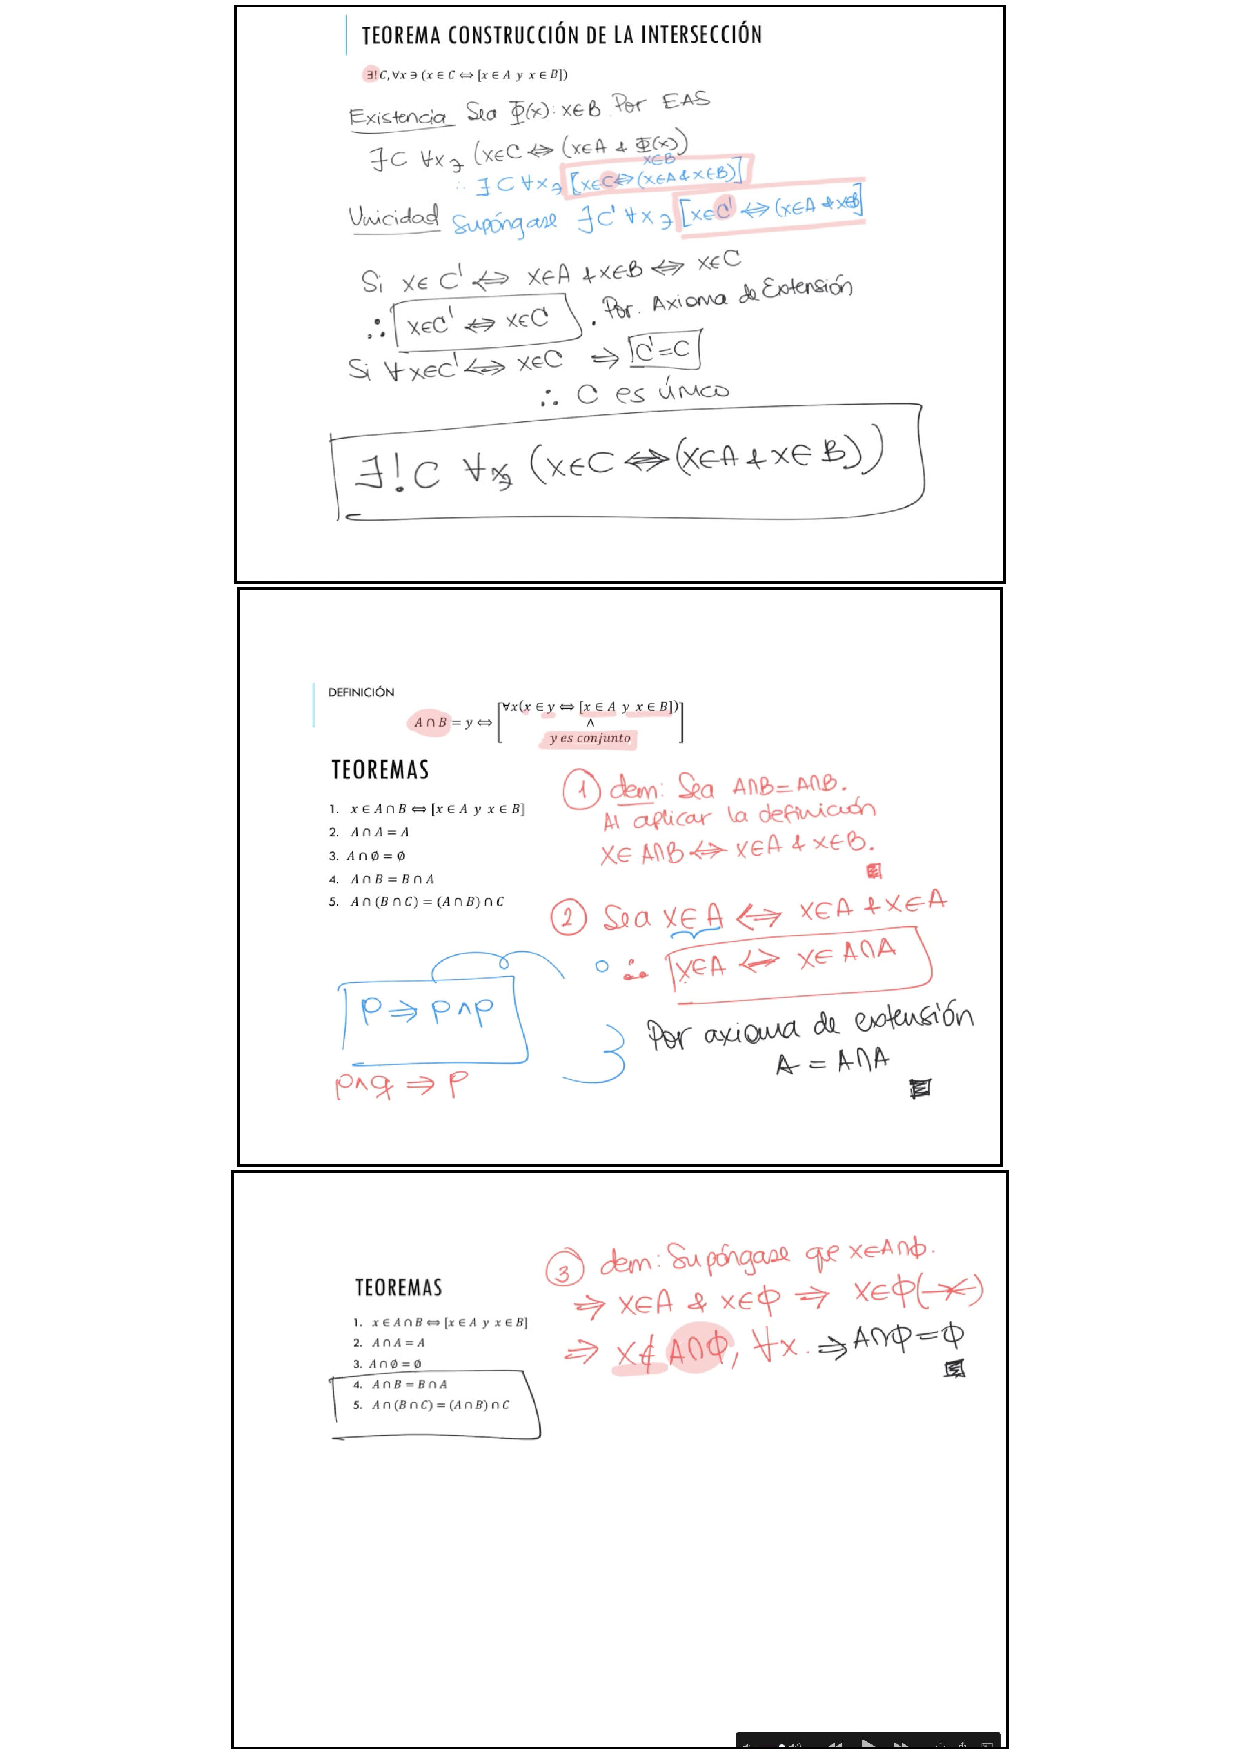
\includepdf[pages=-]{Apendices/s3.pdf}